\documentclass[sigconf,nonacm]{acmart}
\settopmatter{printacmref=false, printfolios=true}
\renewcommand\footnotetextcopyrightpermission[1]{}
\pagestyle{plain}
\usepackage{tikz}
\usetikzlibrary{positioning,arrows.meta,calc,fit}
\usepackage{pgfplots}
\pgfplotsset{compat=1.18}
\usepackage{subcaption}
\usepackage{tabularx}
\usepackage{xcolor}
% Results that depend on the student study and round 4. Every \pending must be gone before submission.
\newcommand{\pending}[1]{\textcolor{red!70!black}{\textbf{[PENDING: #1]}}}

\begin{document}

\title{BridgeFinder}
\subtitle{Finding Research Collaborators Across Communities at UIUC}

\author{Evan Lin}
\affiliation{\institution{University of Illinois Urbana-Champaign}\city{Urbana}\state{IL}\country{USA}}
\author{Eric Liu}
\affiliation{\institution{University of Illinois Urbana-Champaign}\city{Urbana}\state{IL}\country{USA}}

\begin{abstract}
Students who want research experience usually know an instructor in their own area, but few researchers beyond that instructor's circle. BridgeFinder helps them find related researchers in other collaboration communities and shows a chain of co-authors who might introduce them. We built the system on all 102,947 OpenAlex works from UIUC between 2015 and 2024. It detects communities with Louvain, keeps candidates in another community at least three co-authorship steps away, and ranks them by topic overlap plus a bonus for short introduction routes. A three-view web app turns the ranking into a map, a researcher card and an outreach draft. In a historical test on 3,492 researchers, BridgeFinder predicts later cross-community collaborations better than every alternative that searches the same distant pool, including topic matching, degree and path counts, and it ties personalized PageRank while suggesting researchers with six times more topic overlap. Triadic closure still predicts more new ties, and we show that its advantage comes from searching nearby people rather than from a better score. We tested the design with students in four rounds. \pending{one sentence on the student study's headline result and SUS}
\end{abstract}

\keywords{collaboration recommendation, structural holes, co-authorship networks, community detection, research mentoring}

\maketitle

\section{Introduction}
A student who majors in computer science might be drawn to biology, agriculture or public health, but not know anyone who works there. Research experience matters for these students. Undergraduates who take part in research report clearer career plans and stronger research skills~\cite{lopatto2007,hunter2007}, and work that combines distant fields is more likely to have high impact~\cite{uzzi2013}. Yet finding a mentor outside one's own department is hard. UIUC lists 2,574 professor-titled faculty across 110 departments~\cite{graybook}, far too many to browse, and paper search reveals names without telling a student whom they could approach or how to start a conversation.

Social network research suggests where to look. New information tends to arrive through weak ties rather than close friends~\cite{granovetter1973}, and people who bridge structural holes between groups gain access to ideas the groups do not share~\cite{burt1992,burt2004}. A university's collaboration network has many such holes. Groups in different departments can work on related problems for years without writing a paper together~\cite{dahlander2013,barley2025}. BridgeFinder uses this structure directly. A student picks a researcher whose work they already know, such as an instructor. BridgeFinder then suggests researchers in other collaboration communities who work on related topics, and for each one it shows an observed chain of co-authors that could carry an introduction.

The problem is difficult because relevance, novelty and reachability pull in different directions. People who share a co-author with the familiar researcher are easy to find and easy to reach, but they sit inside the circle the student could already discover. People farther away are more likely to be new to the student, yet few of them work on related topics, and the further away they are, the longer and less plausible any introduction becomes. The student also usually has no publications of their own, so the system cannot describe their interests directly. BridgeFinder must find the few distant researchers who are relevant and still reachable through people a student could ask.

We built a working system and evaluated it on real data and with students. This paper makes four contributions.
\begin{itemize}
\item A ranking method that applies brokerage across communities to collaborator discovery, with a candidate rule that excludes the familiar circle by construction and a score that combines topic overlap with a bonus for short introduction routes (Section~\ref{sec:network}).
\item A three-view web application, built for students without publications, that turns each suggestion into a map, a researcher card with an observed introduction route, and an editable outreach draft (Section~\ref{sec:design}).
\item A historical test on 49,651 UIUC papers that compares BridgeFinder against six alternatives on the same candidates and separates the effect of distance from the effect of the score, together with a candid account of where the network analysis falls short (Sections~\ref{sec:network} and~\ref{sec:eval}).
\item Four rounds of student feedback, including a method-blinded rating study, that show how the design changed and whether students find the suggestions relevant, new and worth contacting (Sections~\ref{sec:users} and~\ref{sec:eval}).
\end{itemize}

\section{Related Work}\label{sec:related}
\textbf{Researcher search.} Illinois Experts~\cite{experts} collects institutional profiles, publications and keywords for UIUC researchers. It helps a student check someone's expertise once they have a name, but its keyword search does not consider how researchers are connected, so it cannot show who might introduce the student. Google Scholar~\cite{scholar} covers papers across fields and lets students follow a topic through papers and author profiles, but it also leaves students to work out how to get in contact. Expert-finding models in information retrieval~\cite{balog2006} rank people by how strongly their documents match a query. They are accurate at matching expertise, but they treat each person as a collection of documents and ignore network position. BridgeFinder keeps the research match and adds the route.

\textbf{Referral chains.} ReferralWeb~\cite{kautz1997} linked people whose names appear close together in Web documents and let users explore the resulting social network. A user could ask for their chain of acquaintances to a known researcher, or for colleagues and colleagues of colleagues who know a topic~\cite{perugini2003}. Showing the chain turns an expert into someone the user can reach, which is the idea BridgeFinder borrows most directly. However, ReferralWeb's queries start from the user's own place in the network, so the user must already appear in it, and its colleague answers stay within two links. Students rarely appear in a co-authorship graph, so BridgeFinder starts from a familiar researcher instead and deliberately skips anyone within two links.

\textbf{Literature maps.} Connected Papers~\cite{connectedpapers} draws a visual graph of papers related to a seed paper, which helps when entering an unfamiliar area, and ResearchRabbit~\cite{researchrabbit} supports continued exploration from collections of papers and authors. Both are strong at showing the shape of a literature. Neither shows an introduction route from one researcher to another, and both rank by relatedness rather than by whether a person lies outside the user's existing circle. We adapt their visual exploration to people and possible introductions.

\textbf{People recommendation and link prediction.} Liben-Nowell and Kleinberg~\cite{libennowell2007} compare ways to predict future links from network structure and find that simple measures built on common neighbors, such as the Adamic--Adar score~\cite{adamic2003}, perform well against far more complex ones. LinkedIn's People You May Know~\cite{linkedin} suggests members who share connections, employers or schools, and Twitter's Who to Follow builds each user's candidates with a personalized PageRank walk that starts from that user~\cite{gupta2013}. These systems are accurate and explainable, but they optimize for ties that are likely to form, and likely ties are mostly near the user. This is triadic closure~\cite{easley2010}, the opposite of brokerage. We use shared co-author counts and personalized PageRank as baselines to test what a deliberate move beyond the familiar circle costs and gains.

\textbf{Cross-domain collaboration recommendation.} Tang et al.~\cite{tang2012} learn which topics tend to be linked by cross-field collaborations and rank authors with random walks over author and topic nodes. Their model captures complementary expertise that simple topic matching misses, and it is the closest research system to ours. It represents each person by their publication history, however, while our users usually have none. BridgeFinder uses a familiar researcher's topics as the student's interest proxy, ranks with a fixed and explainable score, and shows a route. Unlike Tang et al., our score does not learn relationships between topics in different fields.

\textbf{Collaboration networks and small worlds.} Newman~\cite{newman2001} showed that scientific collaboration networks are clustered small worlds, in which most pairs of authors are joined by a short chain. Milgram-style experiments show that people can route messages along such chains using only local knowledge~\cite{dodds2003}, and Kleinberg~\cite{kleinberg2000} explains when this decentralized search succeeds. These results suggest that a three-step introduction route is plausible in principle. They do not establish that the people on an observed co-authorship route would actually make an introduction, which we treat as a limitation throughout.

\section{Network Analysis}\label{sec:network}
BridgeFinder rests on two course concepts, brokerage across structural holes and its opposite, triadic closure~\cite{easley2010}. Brokerage is the idea of connecting people in groups that have few ties to one another. A researcher whose collaborators work in many separate groups is in a position to pass ideas between them~\cite{burt1992}. Triadic closure is the tendency of two people with a common friend to become friends themselves. A recommender built on triadic closure suggests people who already share a contact, which keeps suggestions inside the familiar circle. BridgeFinder does the opposite on purpose.

\subsection{Data and graph}
On October 28, 2026, we downloaded all 102,947 OpenAlex~\cite{openalex} works from 2015--2024 that list UIUC (institution \texttt{I157725225}) as an affiliation. The collector pages through the API with a cursor, checks the final count against the API's total, and only replaces the dataset after a complete harvest. We kept the 49,651 works that list at least two different authors affiliated with UIUC on that work, and left out authors from other institutions. Each work also carries up to three OpenAlex topics.

We build an undirected graph whose nodes are UIUC authors and whose edges join two authors who wrote a paper together, weighted by their number of joint papers. To test predictions honestly, everything the system uses comes from 2015--2019 papers, and 2020--2024 papers are held out. Each author's topic profile is their ten most frequent topics in the training papers. Table~\ref{tab:network} describes the training graph.

\begin{table}[t]
\caption{Training co-authorship graph built from 2015--2019 papers.}
\label{tab:network}
\small
\begin{tabular}{@{}lr@{}}
\toprule
Measure & Value\\
\midrule
Authors (nodes) & 19,389\\
Co-authorship edges & 78,281\\
Connected components & 774\\
Largest component share of authors & 87\%\\
Louvain communities & 842\\
Modularity, whole graph & 0.884\\
Modularity, largest component & 0.879\\
\bottomrule
\end{tabular}
\end{table}

\subsection{Communities}\label{sec:communities}
To find the groups a broker would span, we use Louvain~\cite{blondel2008} (networkx, weighted, resolution 1, seed 42). Louvain groups authors who write many papers together by greedily maximizing modularity~\cite{newman2004}, which is high when groups hold more joint papers than chance predicts. The course covered Girvan--Newman~\cite{girvan2002,easley2010}, which instead removes the edge with the highest betweenness again and again until the graph falls apart into groups. We compared both, plus label propagation~\cite{raghavan2007} and greedy modularity~\cite{clauset2004}, on the training graph (Table~\ref{tab:communities}).

\pending{Table and paragraph filled from results/final\_analysis.json, communities part}

\subsection{Choosing suggestions}\label{sec:method}
For a starting researcher $u$, a candidate $v$ must satisfy three rules. It must be in a different community from $u$, it must be reachable from $u$ in the training graph, and its shortest distance from $u$ must be at least three co-authorship steps. The distance rule excludes existing collaborators and anyone who already shares a co-author with $u$, so no suggestion is a triadic-closure suggestion. Reachability guarantees that every suggestion has an observed route to show.

We then rank candidates by
\begin{equation}
\mathrm{Score}(u,v)=S(u,v)+0.5\,\frac{c_3(u,v)}{1+c_3(u,v)}.
\label{eq:score}
\end{equation}
Here $S$ is the Jaccard overlap of the two researchers' topic sets, the number of shared topics divided by the number of distinct topics, or zero if either set is empty. It is a direct use of homophily~\cite{easley2010}, the tendency of similar people to connect. The second term is a path bonus, where $c_3$ counts simple paths $u\to a\to b\to v$ with four distinct people. The bonus saturates, so the first route earns half of the maximum bonus and each extra route adds less, and it stays below 0.5. Ties are broken by author ID, so rankings are deterministic. Path counts and routes ignore edge weights. The coefficient and the saturation are fixed choices, not learned weights. Because they were set during development rather than on held-out data, Section~\ref{sec:validation} tests them on a separate validation split.

The app shows each suggestion's shortest route. If several shortest routes exist, it shows the first one found by breadth-first search from $u$.

\subsection{What the analysis reveals}
For the 50 starting researchers in the app, all 500 suggestions are exactly three steps away, and the path bonus supplies 68\% of their summed scores. The ranking therefore favors people reachable through many short routes over the closest topic match. The 264 distinct intermediaries on the displayed routes sit in broker-like positions. Their median Burt constraint~\cite{burt1992}, computed with edge weights on the largest component, is 0.12, against 0.47 for the median author there. Constraint also drops as people gain collaborators, however, so this alone cannot tell brokers apart from well-connected authors.

Is the path bonus just a popularity score? Across the 3,492 starting researchers of the historical test, the Spearman correlation between a candidate's path count and their number of co-authors, computed within each researcher's distant pool, has a median of only 0.13. BridgeFinder's top-ten suggestions have a median of 9 co-authors, against 146 for a ranking by co-author count alone (Table~\ref{tab:results}). The bonus rewards being reachable from this particular researcher, not being famous in general.

Without the network, the app would lose its community boundary, its distance rule and its introduction routes, and it would become a topic search tool. Section~\ref{sec:eval} shows that both halves of the score matter. Topic overlap alone and path counts alone each predict fewer later collaborations than their sum.

\subsection{Where the network analysis performs poorly}\label{sec:poorly}
We found five weaknesses, which we report here and test in Section~\ref{sec:eval}.

\textbf{Distance costs accuracy.} New collaborations are far more likely between people who already share a co-author. Of the 8,916 new cross-community pairs in 2020--2024, 22\% were two steps apart in the training graph, although two-step candidates are a tiny share of all candidates. The median starting researcher has 29 two-step candidates and 16,290 candidates three or more steps away. Even a random pick from the two-step pool predicts more new ties than BridgeFinder does from the distant pool. Looking past shared contacts is a deliberate trade of accuracy for novelty, and the historical test can only measure the cost, not the benefit.

\textbf{Large teams inflate path counts.} Every co-author of one large paper can receive the same path count from a researcher linked to the team. The 15 training papers with more than 25 UIUC authors produce 8\% of all co-author pairs. This is one reason why 29\% of the 500 displayed suggestions appear on only one UIUC paper between 2015 and 2024. Some of these people are likely students, visitors or outside collaborators.

\textbf{One-paper authors rarely collaborate again.} In the historical test, 27\% of BridgeFinder's top-ten suggestions have a single training paper, and they become new collaborators at a quarter of the rate of the others (0.46\% against 1.77\%).

\textbf{The path bonus can override topic.} Because the bonus supplies most of the score, 14\% of BridgeFinder's top-ten suggestions share no topic with the starting researcher. The midterm grader asked whether such suggestions still feel relevant, which the student study tests (Section~\ref{sec:study}).

\textbf{The graph sees only part of the network.} OpenAlex misses some papers and assigns some affiliations wrongly, our graph leaves out all collaborators outside UIUC, and 11\% of new cross-community pairs had no path at all in the training graph. A co-authorship route also does not confirm that the people on it know each other well or would make an introduction.

\section{System Design and Implementation}\label{sec:design}
\subsection{Goals}
We designed BridgeFinder around four goals that follow from the problem. The student needs no profile or publications of their own (G1). Suggestions must lie outside the familiar researcher's circle (G2). Every suggestion must come with enough evidence for the student to judge relevance themselves, because the score is not a probability (G3). The student must leave with a concrete, low-risk next step (G4).

\subsection{Architecture}
Figure~\ref{fig:pipeline} shows the pipeline. One Python module defines the graph, the communities, the candidate rule and the score, and the app, the historical test and the study cards all import it, so they cannot drift apart. A build step exports the ten suggestions, routes, topics and two example papers for each of the 50 starting researchers to a single JSON file. The app is a static web page that reads this file. It uses D3 for the map and has no server-side logic, so it runs from any static host and works offline. We chose the 50 starting researchers as the six most connected authors with a full list of ten suggestions in each of the eight largest communities, plus the two most connected remaining authors. A student's own instructor may therefore be missing, which we discuss in Section~\ref{sec:limits}.

\begin{figure}[t]
\centering
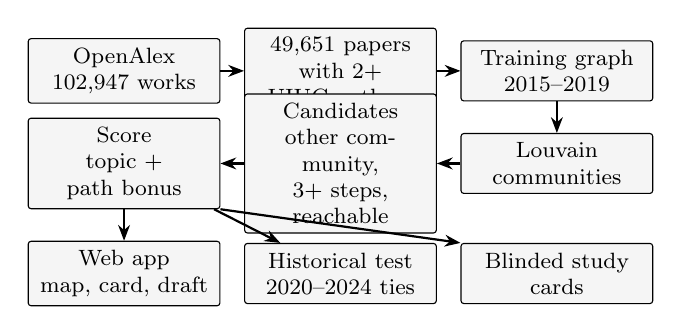
\begin{tikzpicture}[node distance=4mm and 3mm, every node/.style={font=\footnotesize, align=center},
  box/.style={draw, rounded corners=1pt, minimum height=7mm, text width=22mm, fill=black!4},
  arrow/.style={-{Stealth[length=2mm]}, thick}]
\node[box] (oa) {OpenAlex\\102,947 works};
\node[box, right=of oa] (keep) {49,651 papers\\with 2+ UIUC authors};
\node[box, right=of keep] (graph) {Training graph\\2015--2019};
\node[box, below=of graph] (louvain) {Louvain\\communities};
\node[box, left=of louvain] (pool) {Candidates\\other community,\\3+ steps, reachable};
\node[box, left=of pool] (score) {Score\\topic + path bonus};
\node[box, below=of score] (app) {Web app\\map, card, draft};
\node[box, right=of app] (test) {Historical test\\2020--2024 ties};
\node[box, right=of test] (study) {Blinded study\\cards};
\draw[arrow] (oa) -- (keep); \draw[arrow] (keep) -- (graph); \draw[arrow] (graph) -- (louvain);
\draw[arrow] (louvain) -- (pool); \draw[arrow] (pool) -- (score);
\draw[arrow] (score) -- (app); \draw[arrow] (score) -- (test); \draw[arrow] (score.south east) -- (study.north west);
\end{tikzpicture}
\caption{BridgeFinder's pipeline. One shared module builds the graph, communities, candidate pool and score, which feed the app, the historical test and the study cards.}
\Description{A flow diagram from OpenAlex works to retained papers, to the 2015 to 2019 training graph, to Louvain communities, to the candidate pool, to the score, which feeds the web app, the historical test and the study cards.}
\label{fig:pipeline}
\end{figure}

\subsection{The core flow}
Figure~\ref{fig:flow} shows the three views a student moves through.

\textbf{1. Researchers.} The student searches the 50 starting researchers by name or topic, filters by collaboration group or research area, and selects Explore on a researcher card. The landing page explains the three steps in one sentence each. Starting from a familiar researcher meets G1, as in profile search~\cite{experts}, without asking the student for a profile. The proposal let students pick several instructors, but one starting researcher keeps each route short and readable.

\textbf{2. Network.} A map then shows the starting researcher, the ten suggestions and the people on their routes, colored by community (Figure~\ref{fig:flow}b). Solid gray lines are observed co-authorships, and dashed orange lines lead from the starting researcher to each suggestion. A ranked list beside the map names the ten suggestions with their community and route length, and offers the same choices to keyboard and screen-reader users. The visual exploration comes from literature maps~\cite{connectedpapers,researchrabbit}, but the nodes are people. The proposal planned a campus-wide map, but first-round testers found it unreadable (Section~\ref{sec:users}), so the map shows only this neighborhood. Colors are assigned within each view, starting with the selected researcher's community, so no two communities on screen share a color, and a small layout force pushes nodes off lines they do not belong to, so that a line never seems to pass through an unrelated person.

\textbf{3. Suggestions.} Selecting a name or a dashed line opens a researcher card (Figure~\ref{fig:flow}c). Following ReferralWeb~\cite{kautz1997}, the route comes first, as a row of names labeled starting researcher, co-author intermediary and suggested researcher, with a note that the route comes from shared publications and should be checked. Below the route come the suggestion's topics and two example papers, which let the student judge relevance themselves (G3), and a link to their OpenAlex profile. An optional section explains the ranking with the topic overlap, the number of three-step routes and the route bonus. Draft an email opens an editable outreach message that mentions the starting researcher's work, quotes the observed route, and says that the route is not a confirmed personal connection. The student can edit, copy or download it, and nothing is sent automatically (G4).

\begin{figure*}[t]
\centering
\begin{subfigure}[t]{0.32\textwidth}\centering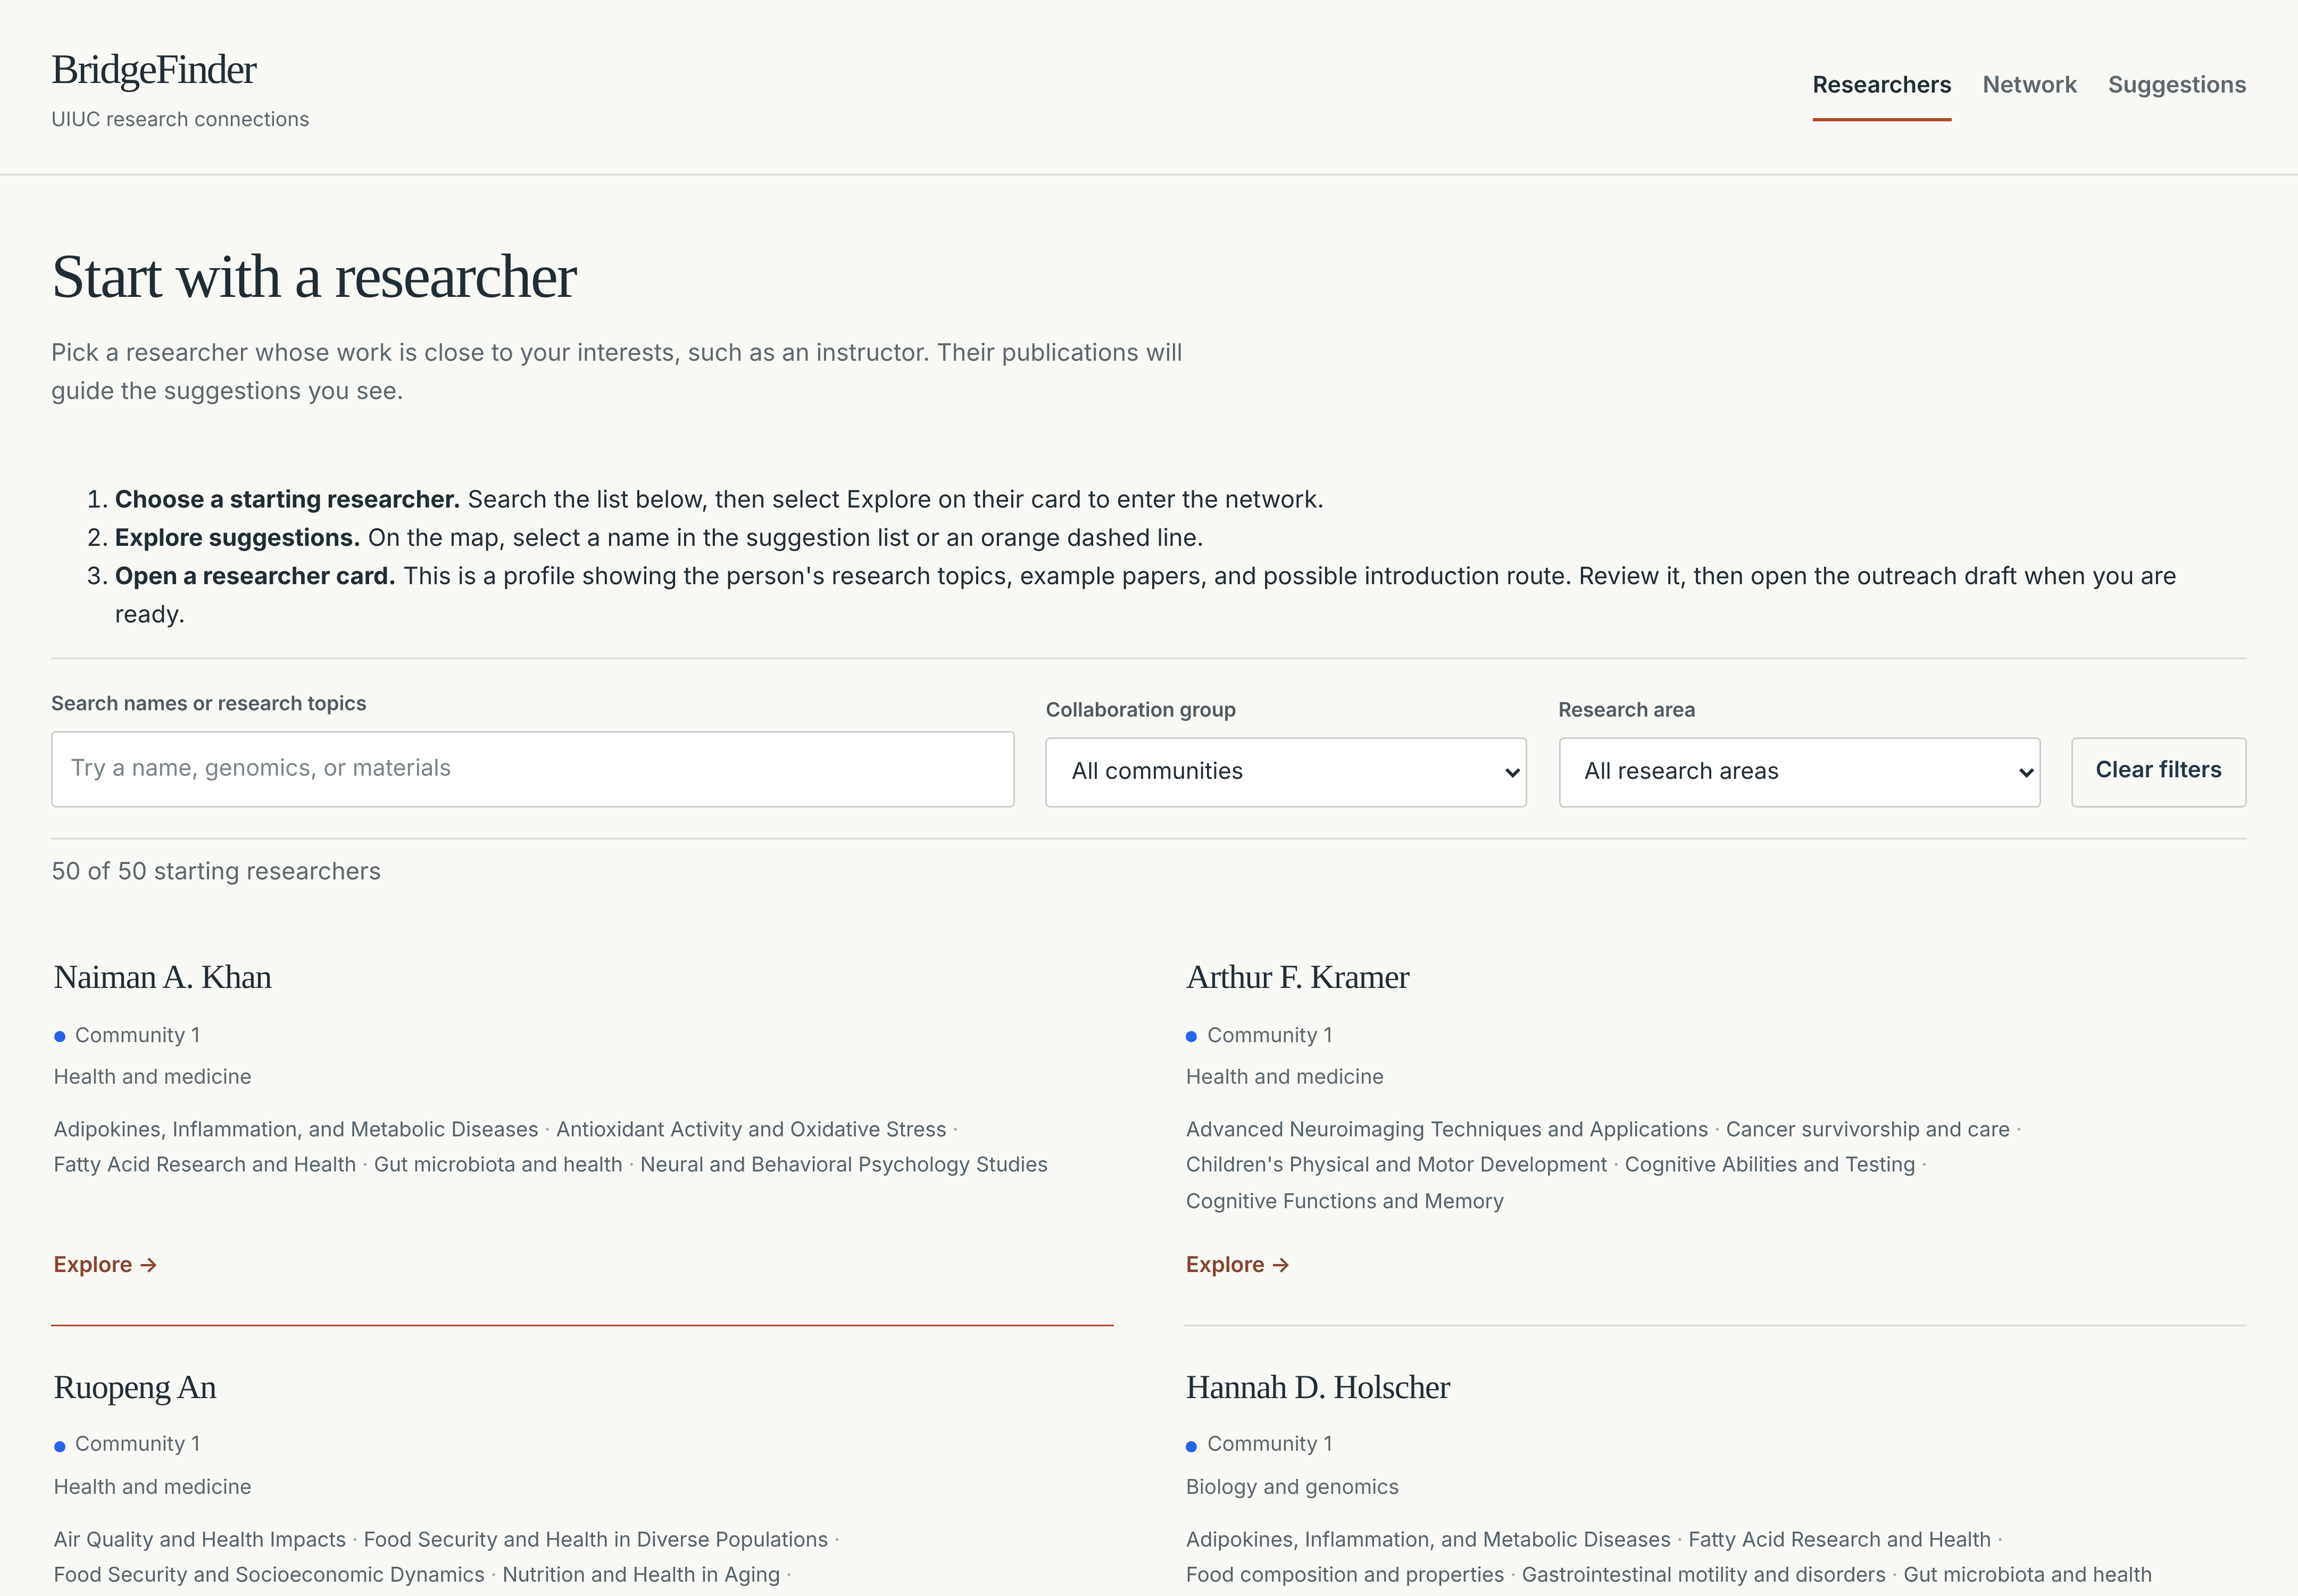
\includegraphics[width=\linewidth,height=5.2cm,keepaspectratio]{figures/01-seeds.png}\caption{Researchers}\end{subfigure}\hfill
\begin{subfigure}[t]{0.32\textwidth}\centering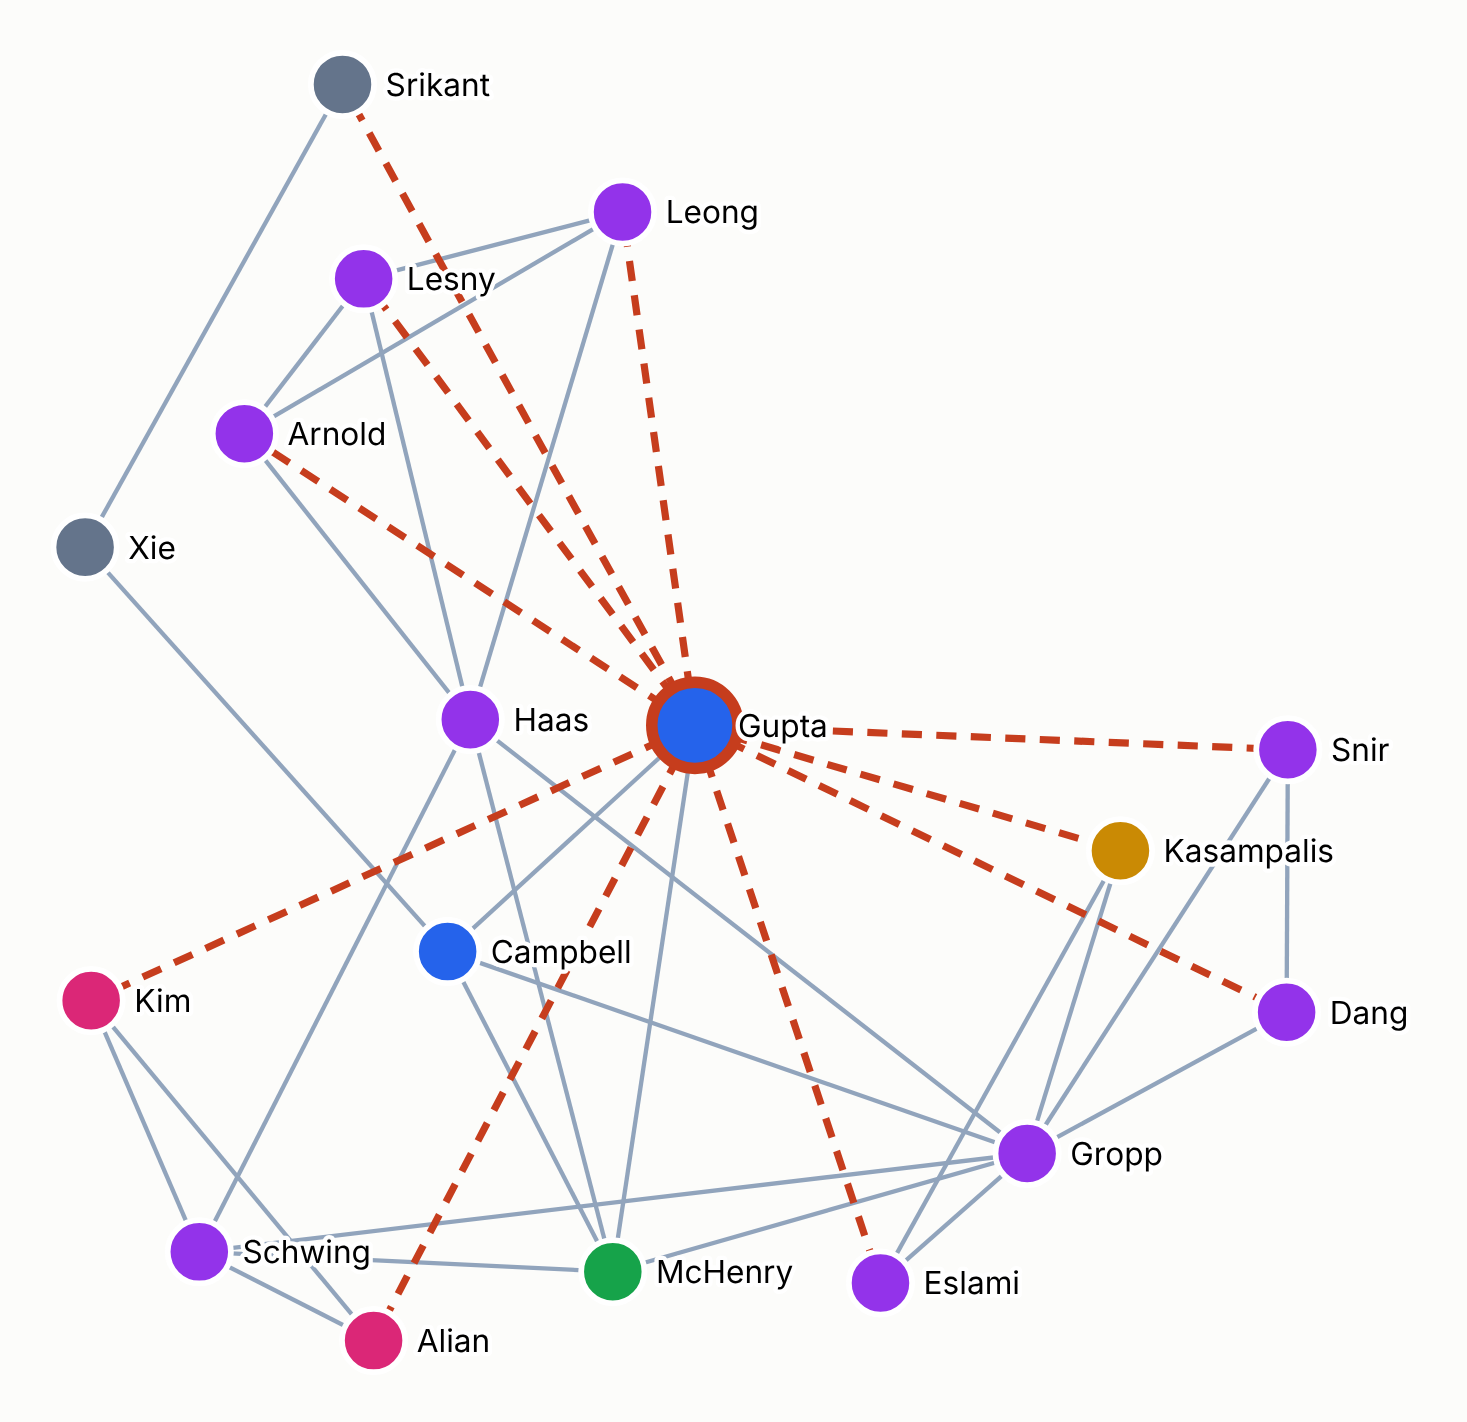
\includegraphics[width=\linewidth,height=5.2cm,keepaspectratio]{figures/02-map.png}\caption{Network}\end{subfigure}\hfill
\begin{subfigure}[t]{0.32\textwidth}\centering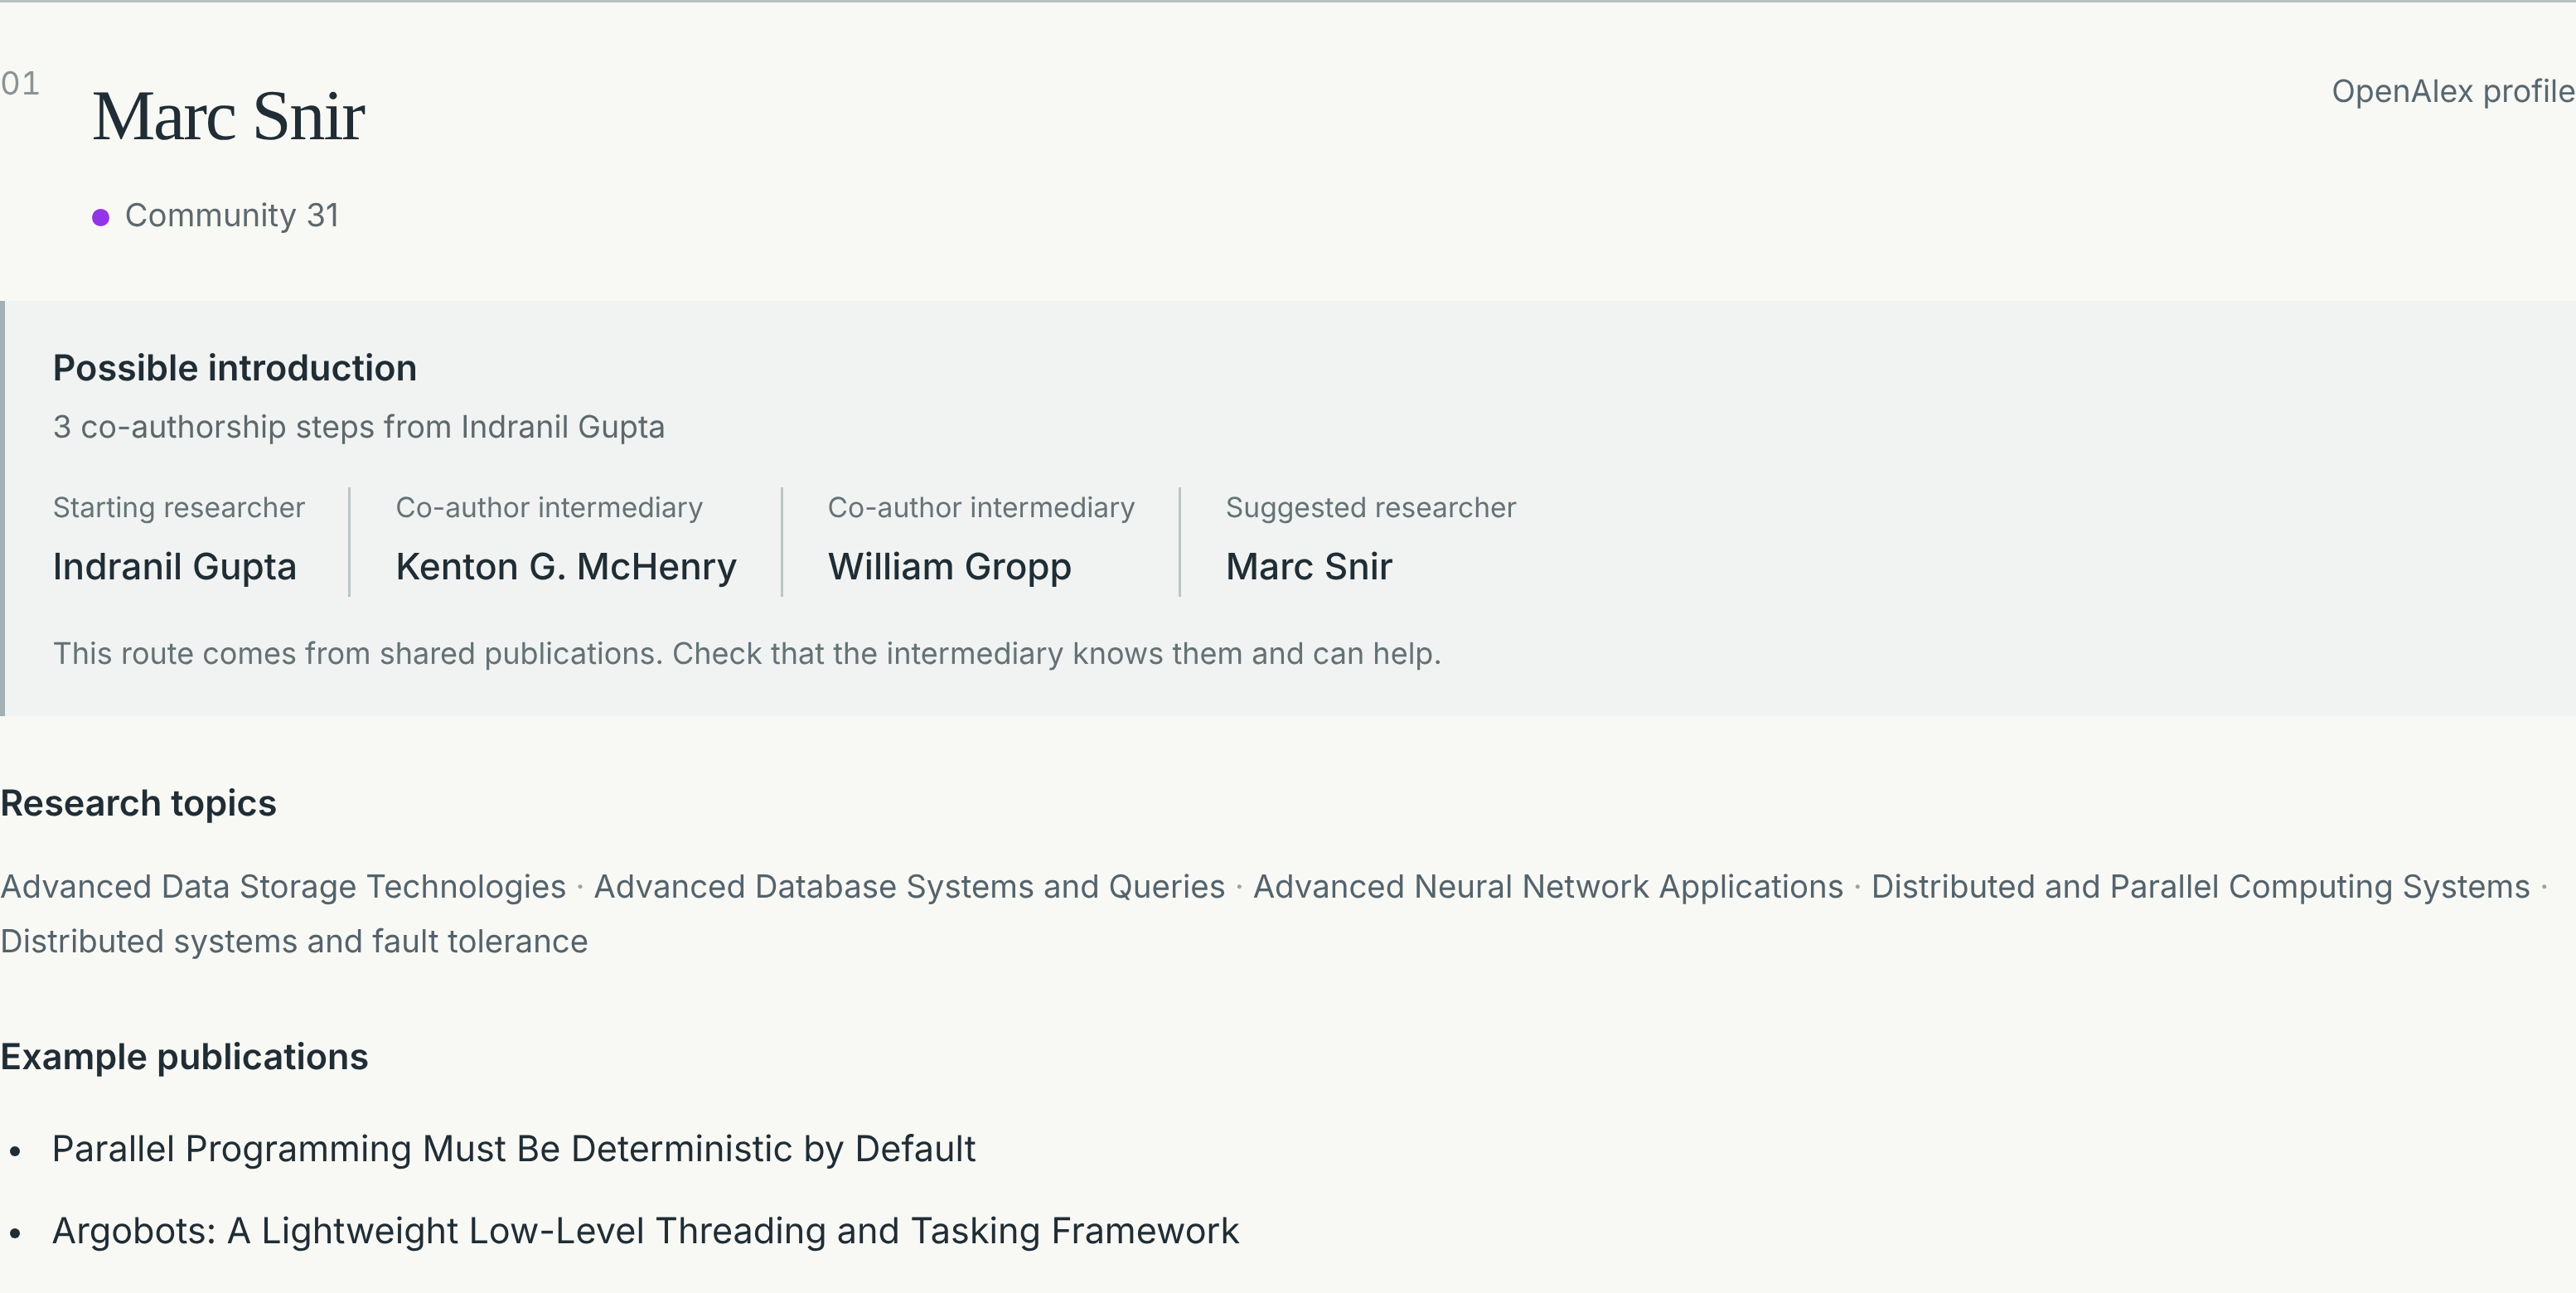
\includegraphics[width=\linewidth,height=5.2cm,keepaspectratio]{figures/03-recommendation.png}\caption{Suggestion card}\end{subfigure}
\caption{The core flow for Indranil Gupta. (a) The student chooses a starting researcher. (b) The map shows observed co-authorships as solid lines and suggestions as dashed lines, colored by community. (c) The card for Marc Snir, the top suggestion, shows the route through Kenton G. McHenry and William Gropp, then topics and example papers. The route is observed in publications and is not a confirmed introduction.}
\Description{Three screenshots of the BridgeFinder app. The first shows a grid of starting researchers with a search box. The second shows a network map with a ringed central node, dashed lines to ten suggested researchers and solid lines between co-authors. The third shows a researcher card with an introduction route of four names, topic tags and example publications.}
\label{fig:flow}
\end{figure*}

\subsection{Design decisions and where they came from}
Table~\ref{tab:decisions} traces the main decisions to the problem, to related work or to what we learned from users. Two decisions came from our own analysis rather than from users. Requiring a route (reachability) is a change from the proposal's mock-up, made so that every card can show one. Showing topics and papers under the route came from finding that the path bonus dominates the score, so the card must give the student the evidence to reject a weak topic match.

\begin{table}[t]
\caption{Main design decisions and their sources.}
\label{tab:decisions}
\small
\begin{tabularx}{\columnwidth}{@{}>{\raggedright\arraybackslash}X>{\raggedright\arraybackslash}p{0.38\columnwidth}@{}}
\toprule
Decision & Source\\
\midrule
Start from a familiar researcher & Students have no papers (G1), Tang et al.~\cite{tang2012}\\
Skip anyone within two steps & Brokerage over triadic closure (G2)\\
Route first on the card & ReferralWeb~\cite{kautz1997}\\
Map of people, not papers & Literature maps~\cite{connectedpapers}\\
Focused map, not campus-wide & Round 1 feedback\\
Landing-page steps, card definition & Round 1 feedback\\
Separate research areas from communities & Round 1 feedback\\
Topics and papers under the route & Path bonus dominates (Section~\ref{sec:network})\\
Editable draft, never sent & G4, trust in the route\\
\pending{decisions from rounds 3 and 4} & Rounds 3 and 4\\
\bottomrule
\end{tabularx}
\end{table}

\subsection{Reproducing the system}
The repository contains the collector, the dataset with its completeness record, the shared model, the app and the study tools. Running the collector, then the web-data export, then a static file server reproduces the app exactly, because every ranking is deterministic. Each result file in the paper carries a manifest with hashes of the dataset and the code that produced it, and unit tests check the model against hand calculations, check every displayed route and ranking for all 50 starting researchers, and check that every number in this paper matches the result files.

\section{Users and Feedback}\label{sec:users}
Our target users are UIUC undergraduates and early-stage graduate students who want research experience but have few contacts beyond their classes or department. They are the people who lack the network BridgeFinder supplies, and they can judge whether a suggestion is relevant and new to them in a way no historical test can. We tested the design with students in four rounds (Table~\ref{tab:rounds}).

\begin{table*}[t]
\caption{Feedback rounds. Each round tested the version produced by the previous one.}
\label{tab:rounds}
\small
\begin{tabularx}{\textwidth}{@{}l>{\raggedright\arraybackslash}p{0.2\textwidth}>{\raggedright\arraybackslash}X>{\raggedright\arraybackslash}X@{}}
\toprule
Round & Students & What they did & What changed\\
\midrule
1 (before midterm) & 4, two graduate and two undergraduate, in CS, computational biology, ECE and Food Systems & Worked through the first prototype with minimal context and reported problems as they met them & Landing-page steps, renamed views, focused map, corrected labels\\
2 (before midterm) & 6, two undergraduate and four master's students, in mathematics and CS, CS and business technology management & Reviewed the revised app & No new problems, so no changes\\
3 (after midterm) & \pending{N, composition} & Used the app on their own, then rated method-blinded suggestion cards and completed the SUS & \pending{changes}\\
4 & \pending{N} & \pending{what they did} & \pending{changes confirmed}\\
\bottomrule
\end{tabularx}
\end{table*}

\textbf{Round 1.} The first round had two graduate students, one in Computer Science and one a Master of Computer Science student researching computational biology, and two undergraduates, one in Electrical and Computer Engineering and one in Food Systems. Together they cover both levels we target. The Food Systems student represents the non-computing side of the cross-field searches BridgeFinder targets, and the computational biology student has already made such a move. We gave each student minimal context in an individual session and asked them to work through the app, and they gave feedback as they ran into problems. Four students is below the five to ten the proposal cited, but small formative rounds can expose major problems before a larger study~\cite{nielsen1993}. We made four changes.
\begin{itemize}
\item \textbf{Getting started.} One student looking for a relevant professor did not realize they first had to choose a researcher to enter the graph. We added landing-page instructions to choose a starting researcher, explore a suggestion and review its route.
\item \textbf{Understanding the interface.} Students found the interface unintuitive, so we simplified the layouts and named the three views Researchers, Network and Suggestions. Students were also unsure what a card meant, so the landing page now defines a researcher card as a profile with topics, example papers and a possible introduction route, and the map legend distinguishes observed collaborations from suggestions.
\item \textbf{Readable map.} The campus-wide graph showed too many nodes to follow, so we narrowed the map to the selected researcher, the suggestions and the people on their routes.
\item \textbf{Correct labels.} Some tags did not match the researchers shown. We corrected the profile labels and now distinguish inferred research areas from collaboration communities.
\end{itemize}

\textbf{Round 2.} Six more UIUC students then reviewed the revised app. Two were undergraduates studying mathematics and computer science, one in a dual degree and one in the combined degree. Three were Master of Computer Science students, and one was a master's student in business technology management. All six found the revised interface clear, raised no new problems, and approved of the app. Most testers in the first two rounds study computing, so for the third round we recruited across the five research areas of the study's starting researchers.

\textbf{Round 3.} \pending{composition and recruitment of the study participants, by level and field, and how many were moderated or self-guided}. Each student first wrote a research interest in their own words, then used the app on their own with the task of finding someone they might write to. We recorded what they did. In self-guided sessions the study page logged which views they opened, which suggestions and cards they chose, whether they opened the ranking explanation and the outreach draft, and how long they spent, but never the text of their draft. After the task, students answered three questions about what the solid lines, the dashed lines and the route mean, then rated suggestion cards and completed the System Usability Scale~\cite{brooke1996}, and finally described what confused them, whether they would contact anyone, how far they trusted the route, and what they would change. \pending{what students actually did, from the event logs and notes, for example how many reached a card and a draft without help, where they hesitated, what they misread}. \pending{the changes made in response}

\textbf{Round 4.} \pending{a short check of the round-3 changes with new students, using the same unaided task and debrief}.

\section{Evaluation}\label{sec:eval}
We evaluate BridgeFinder in two ways. A historical test asks whether its suggestions anticipate real collaborations, and a student study asks whether students find them relevant, new and worth contacting. Table~\ref{tab:metrics} lists the metrics, why each matters and its baseline.

\begin{table}[t]
\caption{Metrics, reasons and baselines.}
\label{tab:metrics}
\small
\begin{tabularx}{\columnwidth}{@{}>{\raggedright\arraybackslash}p{0.27\columnwidth}>{\raggedright\arraybackslash}X>{\raggedright\arraybackslash}p{0.27\columnwidth}@{}}
\toprule
Metric & Why & Baseline\\
\midrule
P@10 on 2020--2024 ties & The app shows ten suggestions, and a later co-authorship is the strongest available sign of a useful match & Triadic closure, Topic-Only, PageRank, degree, path count, random\\
Relevant and new (share of cards rated 5 or more on both) & The core claim, that BridgeFinder finds relevant people the student did not know & Triadic closure (primary), Topic-Only\\
Willingness to contact & Whether the route makes contact feel realistic & Topic-Only\\
Task completion and route understanding & Whether students can use the flow and read the route correctly & Target of 12 of 15\\
SUS & Overall usability & Published norms~\cite{bangor2008}\\
\bottomrule
\end{tabularx}
\end{table}

\subsection{Historical prediction}\label{sec:historical}
We built the graph, communities and topic profiles from 2015--2019 papers and asked which starting researchers formed new cross-community collaborations in 2020--2024. A new tie is a co-authorship in 2020--2024 between two training-graph authors in different communities who had not written together before. We evaluated all 3,492 starting researchers with at least one such tie. For each method we take its first ten suggestions and compute P@10, the share of them who became new collaborators, along with recall at ten, NDCG at ten and the hit rate, the share of researchers with at least one correct suggestion. We divide hits by ten even when fewer suggestions exist.

The midterm compared BridgeFinder with triadic closure, but the two methods search different pools, so the comparison could not separate the effect of distance from the effect of the score. Here every method on the same line of Table~\ref{tab:results} ranks the same candidates. The distant pool holds BridgeFinder's candidates, people in another community three or more steps away. The two-step pool holds triadic closure's candidates, people in another community who share at least one co-author with the starting researcher. Besides BridgeFinder and triadic closure, we test the course's PageRank~\cite{brin1998,easley2010} in its personalized form, which restarts every walk at the starting researcher~\cite{haveliwala2002,gupta2013} (damping 0.85, weighted edges), the number of co-authors as a pure popularity baseline, each half of Equation~\ref{eq:score} alone, and the exact expectation for a random ranking. We compare methods with a paired bootstrap over researchers (2,000 resamples).

\begin{table*}[t]
\caption{Historical prediction of new 2020--2024 cross-community collaborations for 3,492 starting researchers. Methods within a pool rank the same candidates. The last two columns describe each method's top-ten suggestions.}
\label{tab:results}
\small
\begin{tabular}{@{}llrrrrrr@{}}
\toprule
Pool & Method & P@10 & R@10 & NDCG@10 & Hit rate & Median co-authors & Topic overlap\\
\midrule
Distant (3+ steps) & BridgeFinder & \textbf{0.0131} & \textbf{0.0350} & \textbf{0.0264} & \textbf{0.111} & 9 & 0.196\\
 & Personalized PageRank & 0.0129 & 0.0311 & 0.0260 & 0.104 & 31 & 0.032\\
 & Path count only & 0.0090 & 0.0231 & 0.0183 & 0.079 & 27 & 0.028\\
 & Topic-Only & 0.0079 & 0.0209 & 0.0156 & 0.066 & 4 & 0.283\\
 & Co-author count & 0.0052 & 0.0061 & 0.0062 & 0.046 & 146 & 0.003\\
 & Random (expected) & 0.0002 & 0.0004 & 0.0003 & 0.002 & & \\
\midrule
Two-step & Personalized PageRank & \textbf{0.0340} & \textbf{0.0914} & \textbf{0.0790} & \textbf{0.245} & 31 & 0.062\\
 & Triadic closure (shared co-authors) & 0.0287 & 0.0806 & 0.0652 & 0.214 & 21 & 0.062\\
 & BridgeFinder score & 0.0269 & 0.0811 & 0.0634 & 0.200 & 14 & 0.145\\
 & Topic-Only & 0.0243 & 0.0757 & 0.0579 & 0.187 & 11 & 0.148\\
 & Random (expected) & 0.0167 & 0.0543 & 0.0366 & 0.138 & & \\
\bottomrule
\end{tabular}
\end{table*}

\textbf{BridgeFinder is the best ranking of distant candidates.} Within the distant pool, BridgeFinder's P@10 of 0.0131 is 65 times the random expectation and higher than co-author count (difference 0.0079, 95\% CI 0.0063 to 0.0095), path count alone (0.0041, CI 0.0028 to 0.0055) and topic overlap alone (0.0052, CI 0.0040 to 0.0064). Topic overlap and path count each carry signal, and their sum predicts better than either. Personalized PageRank ties BridgeFinder (difference 0.0002, CI $-$0.0014 to 0.0018), but the two reach the same accuracy with different people. PageRank's suggestions have a median of 31 co-authors and a mean topic overlap of 0.032, while BridgeFinder's have 9 co-authors and an overlap of 0.196. For a student, a suggestion's research has to match their interest, so at equal accuracy we prefer the ranking whose suggestions share six times more topics. This is the evidence behind our choice of the score over the PageRank covered in class.

\textbf{The gap to triadic closure comes from distance, not the score.} Triadic closure's P@10 of 0.0287 is more than twice BridgeFinder's, as in the midterm. On the two-step pool, however, BridgeFinder's score reaches 0.0269, almost the same as triadic closure (difference 0.0018, CI 0.0001 to 0.0036). The score is about as good as counting shared co-authors at ranking nearby people. What costs accuracy is the decision to look three or more steps away, where the median researcher has 16,290 candidates and only two of them become new collaborators. That decision is the point of BridgeFinder, because the nearby people are exactly those a student could find through the familiar researcher.

\textbf{The best predictor stays near the familiar circle.} Personalized PageRank over all reachable candidates has the highest P@10 of all (0.0369), because its top suggestions are almost all two steps away. This confirms the tension in Section~\ref{sec:network}. A system tuned only for predicting collaborations would recommend the familiar circle.

\subsection{Validation of the fixed choices}\label{sec:validation}
\pending{validation sweep paragraph and figure from results/final\_analysis.json, validation part}

\subsection{Student study}\label{sec:study}
\textbf{Design.} Each student first states a research interest, uses the app as described in Section~\ref{sec:users}, and then picks the closest of five starting researchers, one from each of the five largest communities, covering nutrition and metabolic health, crops and bioenergy, materials and sensors, sensor networks and network analysis, and maternal health. The student then rates every card for that researcher, 13 to 15 cards in random order with method labels hidden. Each method contributes its own top five. A candidate chosen by two methods appears once and counts for both. All cards use the same fields and the same shortest-route procedure. Triadic closure cards necessarily show two-step routes, so blinding is only partial for that comparison. Students rate each card from 1 to 7 on relevance to their stated interest, on how new the person is to them, and on how realistic contact feels given the route. The primary outcome is the share of cards rated at least 5 for both relevance and novelty, compared between BridgeFinder and triadic closure within each student with a paired Wilcoxon test. Other comparisons are exploratory with Holm correction. Students could take part in a moderated session or through a self-guided version of the same study, a single web page that includes the app and returns the answers as text the student pastes back to us. Both versions use identical cards, questions and scales.

\textbf{Results.} \pending{Table of mean relevance, novelty, willingness to contact and relevant-and-new share per method, with the primary comparison, its confidence interval and p-value, and the Topic-Only comparisons. Then task completion, route understanding and SUS against their targets.}

\textbf{Do low-overlap suggestions still feel relevant?} \pending{The grader's question. BridgeFinder's study cards range in topic overlap from 0.05 to 0.23. Report mean relevance for its cards below and above the median overlap of 0.125, the within-student correlation between overlap and relevance, and what this implies for the path bonus.}

\subsection{What did not work}
BridgeFinder did not meet the proposal's goal of predicting more new collaborations than both baselines. Triadic closure predicts more, and personalized PageRank across all distances predicts more still. Section~\ref{sec:historical} shows that this follows from the distance rule rather than from the score, but the historical test cannot show that the extra novelty is worth the lost accuracy. Only students can judge that. The path bonus also lets weak topic matches and one-paper authors into the top ten (Section~\ref{sec:poorly}). \pending{study findings that did not meet their targets}

\section{Discussion and Limitations}\label{sec:limits}
\pending{Revise once study results are in.} Our results describe a trade-off that any brokerage recommender faces. Nearby people are the safest prediction, and a student can usually find them already. Distant people are new, but few of them collaborate later, and the historical record cannot say whether a suggestion that never led to a paper was nonetheless useful to a student. BridgeFinder's score makes the distant pool as predictable as the network allows. It matches PageRank's accuracy with researchers whose work is much closer to the starting researcher's.

Several limitations remain. A co-authorship route does not show that the intermediaries know each other well, would introduce a student, or that the suggested researcher is available to mentor. Our graph misses ties to authors outside UIUC and collaborations that never produced a paper, and OpenAlex affiliations and dates add noise. Of the 500 displayed suggestions, 29\% appear on only one UIUC paper between 2015 and 2024, and one paper does not establish a current UIUC appointment. The 50 starting researchers are highly connected authors in large communities, so a student's own instructor may be missing, and the starting researcher's topics only approximate the student's interests. The study's method key is stored in our public repository, although it is never shown to participants and no student could see it while rating. \pending{study limitations, such as sample size, field mix and self-guided versus moderated sessions}

Two changes follow directly from this work. A minimum of two UIUC papers per suggestion would remove most one-paper authors, and Section~\ref{sec:validation} tests it on validation data before any change to the app. Letting students start from their own instructor, rather than one of 50 researchers, would require precomputing suggestions for every author, which the shared model already supports.

\section{Conclusion}
BridgeFinder helps students look beyond the researchers they already know. On ten years of UIUC publications, its combination of topic overlap and introduction routes is the most accurate way we found to rank people three or more steps away, matching personalized PageRank while suggesting people whose research is much closer to the student's starting point. Looking that far away costs accuracy against triadic closure, which stays inside the familiar circle. \pending{one or two sentences on what students said, from the study}

\section*{Contributions}
Evan Lin built the app and ran the analysis. Eric Liu ran the user testing.

\section*{AI Use}
We used Claude for early development of the prototype, to draft early versions of the reports, and to write analysis scripts for the final report. We also used Perplexity and OpenAI Codex to check the work and revise it. We read and verified everything ourselves, and every number in this paper is checked against the result files by automated tests.

\bibliographystyle{ACM-Reference-Format}
\bibliography{references}

\end{document}
